\documentclass[twoside,11pt]{article}

% Any additional packages needed should be included after jmlr2e.
% Note that jmlr2e.sty includes epsfig, amssymb, natbib and graphicx,
% and defines many common macros, such as 'proof' and 'example'.
%
% It also sets the bibliographystyle to plainnat; for more information on
% natbib citation styles, see the natbib documentation, a copy of which
% is archived at http://www.jmlr.org/format/natbib.pdf

\usepackage{jmlr2e}
\usepackage{makecell}
%\usepackage{parskip}
\usepackage{hyperref}
\usepackage{subfigure}

% Definitions of handy macros can go here
\newcommand{\dataset}{{\cal D}}
\newcommand{\fracpartial}[2]{\frac{\partial #1}{\partial  #2}}
% Heading arguments are {volume}{year}{pages}{submitted}{published}{author-full-names}

% Short headings should be running head and authors last names
\ShortHeadings{95-845: AAMLP Article}{Kainosho and Townsend}
\firstpageno{1}

\begin{document}

\title{Heinz 95-845: Classifying Obesity in Children Using Demographic Survey Data \\ Applied Analytics: the Machine Learning Pipeline}

\author{Atsumi Kainosho\qquad Haley Townsend\\
\em Carnegie Mellon University, Heinz College}\

\maketitle
\vspace{1em}
\begin{abstract}
   Childhood obesity in the United States constitutes a national health emergency. The Centers for Disease Control and Prevention (CDC) wants to tackle this problem with improved policy strategies. To better inform their policy-making efforts, we built multiple machine learning models to classify children's BMI category, obese versus not. We use data on 1,576 participants from the 2012 NHANES National Youth Fitness Survey, managed by the CDC. Our best baseline model (AUC of 0.617), a logistic regression, uses gender, age, race and birth country to classify BMI category. To boost performance, we added two features to this baseline model: income and number of young children in the household. This improved performance slightly (AUC of 0.659) with the highest performing model being the gradient boosted forest. This study demonstrates the ability to improve model performance by adding the right new features. Agencies like the CDC can glean insights from models using only demographic features in their classifications, but these results should be supplemented with other sources.
 
\end{abstract}


\section{Introduction}\label{intro}
Advances in machine learning classification methods have resulted in substantial progress across countless domains, especially those in the private sector. However, public sector agencies tend to lag behind their private sector counterparts in terms of complex data analyses. This work attempts to narrow some of that gap. Specifically, we aim to provide methods and insights to the Centers for Disease Control and Prevention (CDC) and other health protection agencies. The overall purpose of this project is to apply the entire machine learning pipeline to observational data. In particular, we use demographic survey data to classify Body Max Index (BMI) category in U.S. children. 

Machine learning is taking off in health fields. For example, \cite{zheng:17} used classification models to identify Type 2 diabetes from electronic health records. \cite{horn:17} validated a classification model detecting colorectal cancer cases using basic demographic data as well as colonoscopy and blood count data. Additionally, \cite{maenner:16} constructed a machine learning algorithm to monitor autism spectrum disorder (ASD), which was later submitted to the CDC to improve their baseline methods. Finally, \cite{bergquist:17} applied ensemble methods to classify lung cancer severity using health care claims data. However, all four of these recent studies used detailed health records and medical claims data to build their high-performing models. More often than not, the CDC does not have access to an individual's entire medical history. Even if they did, the amount of information would be overwhelming and extremely difficult to parse through. 

Therefore, we explored research incorporating broader, demographic data instead of detailed health records, specifically with respect to adolescent obesity and BMI. \cite{cockrell:18} provided updated prevalence estimates on U.S. adolescent obesity trends by using adjusted Wald tests and ordinary least squares linear regression. Notably, they used data from the CDC's National Health and Nutrition Examination Surveys (NHANES) over seven years to construct their estimates. Our work in this paper uses similar, but more recent data from the same source. \cite{kaur:17} also called upon NHANES data in their associational study between obesity and food insecurity. They used simple logistic regressions to find these associations. Additionally, \cite{heer:16} evaluated the association between adverse family experience during childhood and later obesity by performing a cross-sectional analysis of the 2012 National Survey of Children's Health.  Finally, \cite{ohri:13} assessed the relationship between food, physical activity and environment with a child's weight status by applying multivariate analysis on survey data collected on children living in low-income New Jersey cities. While these three studies used observational survey data to inform their methods, none of them employed sophisticated machine learning techniques beyond logistic or linear regression. 

While the first four studies mentioned employed sophisticated machine learning methods in their analyses, the latter four studies did not. However, the latter four studies used demographic survey data while the first four studies used detailed, often unobtainable health records in their model-building. Therefore, we seek to bridge the gap between these two sets of studies and apply machine learning classification methods to accessible demographic survey data. 

Section \ref{background} reviews the problem context in greater depth. Section \ref{model}, describes and explores the data, explains the machine learning methods used and describes the evaluation criteria. Section \ref{results} reports the main results of our analysis. Section \ref{discussion} provides additional discussion and suggests avenues for future work. Section \ref{conclusion} summarizes the key contributions of this paper and brings the study full circle. Finally, the Appendices review specifics of the data, data missingness and the application of neural networks in this study. 

\section{Background} \label{background}
Body Mass Index (BMI) - a standardized weight-to-height ratio - is a common and informative metric used by the Centers for Disease Control and Prevention (CDC), the nation's health protection agency. This indicator is often used to flag individuals who could have an unhealthy level of fat. Being overweight can lead to many health consequences and/or exacerbate existing conditions, such as diabetes. Therefore, reducing the number of overweight and obese persons in the country constitutes a top priority for the CDC. Specifically, the CDC states: {\em Our obesity efforts focus on policy and environmental strategies to make healthy eating and active living accessible and affordable for everyone.}

Understanding this priority, our goal is to provide important structure and insights to the CDC. For example, the CDC could use our classifier to better target at-risk youth with additional health assistance (e.g. more food stamps). This project aims to not only provide insights and recommendations from the results, but also showcase the entire machine learning pipeline for this specific context. Which, as mentioned in the previous section, has not been performed in the context of health survey data for the CDC beyond basic regression. While we will be performing this analysis on data from the CDC, we intend for this pipeline to serve other health and nutrition agencies as well. Officials in health care fields can detect potentially unhealthy children based only on their socio-demographic backgrounds. They can use these results to better inform their health care policy efforts. 


\section{Methods: Applying Known Models to a New Context}\label{model}
Our study does not introduce new mathematical or statistical methods. Instead, we combine existing methods and apply them in a new context. Therefore, this section describes the data we used to construct our models and explains the evaluation criteria used to compare performance across models. The complete code is available at \url{https://github.com/AtsumiNK/ML-Final-Project}.

\begin{figure}[h]
  \centering 
  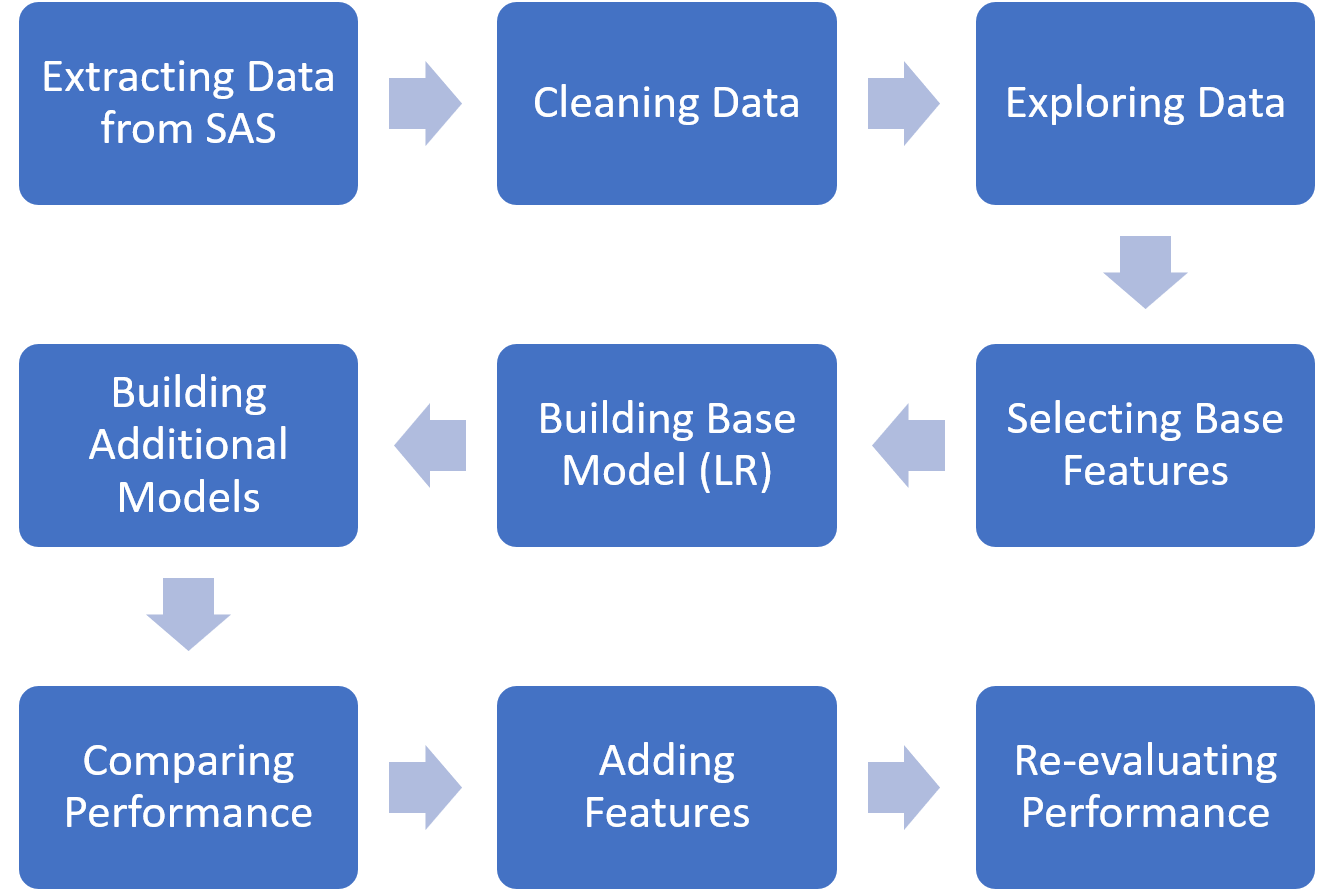
\includegraphics[width=6in]{flow_chart_process_2.png} 
  \caption{Methodology Work Flow}
  \label{fig:example} 
\end{figure} 

\subsection{Data Extraction} 
We used publicly available data from the 2012 National Health and Nutrition Examination Survey (NHANES) National Youth Fitness Survey (NNYFS) for this study. This data is observational and comes from a self-reported survey. This one-time survey collected demographic, dietary, health and examination data on 1,576 children ages 3 to 15 years old across the United States. Specifically, these children are part of the non-institutionalized, resident population and are considered {\em nationally representative.}

The outcome variable of interest for our study is Body Mass Index (BMI) category, which we re-leveled slightly to create a binary outcome indicating whether the child is categorized as obese or not. Five of the subjects were missing the outcome, BMI, in the data. Therefore, we immediately removed these five rows of data. Please see Appendix B for an additional discussion on the handling of missing values and imputation. The BMI category variable originates from the {\em Examination} data in the {\em Body Measures} file. The covariates originate from the {\em Demographics} data in the {\em Demographic Variables and Sample Weights} file. During the analysis process, we experimented with other covariates from the {\em Diet} file, including energy and fat intake. However, given our intended use case, we decided to stick to demographic predictors only since health agencies generally will not have access to precise diet data.

\subsection{Data Cleaning and Exploration}
We used data from two main SAS files, which are publicly available at the CDC website's \href{ https://wwwn.cdc.gov/nchs/nhanes/search/nnyfs12.aspx}{National Health and Nutrition Examination Survey page}. The first file contains data on subject demographics. The second contains physical examination data on body measures. From the second file, we only included one variable, the outcome variable: BMI Category. Originally, this variable had four levels, other than missing: (1) underweight, (2) normal weight, (3) overweight and (4) obese. However, we re-leveled this to be a binary variable of either obese or not (combining underweight, normal weight and overweight). 

Table 1 shows descriptive statistics of the features selected for model-building, which include gender, age, race, birth country, annual household income and the number of children in the household 5 years old or younger. For the baseline models, however, we only included gender, age, race and birth country. Table 2 describes the baseline features, including the outcome variable, in more detail. These baseline features are easily accessible for health agencies and closely align with the features used in the baseline logistic regression model from a previous study, which will be discussed in the next Section, \ref{lr}. 

\renewcommand\theadalign{bc}
\renewcommand\theadfont{\bfseries}
\renewcommand\theadgape{\Gape[4pt]}
\renewcommand\cellgape{\Gape[4pt]}

\begin{table}[h]
 \begin{minipage}[h]{.45\textwidth}
  \begin{center} 
   \begin{tabular}{| c  c  r| } 
    \hline
    \thead{Variables} & {} &{}\\
    \hline \\[-11pt]

    BMI &  \makecell{N\\Y} & \makecell{1,227\\299}  \\ 
    \hline
    gender & \makecell{male\\female} & \makecell{768\\758}  \\
    \hline
    age & \makecell{Min\\1st Qu\\Median\\Mean\\3rd Qu\\Max} & \makecell{3.00 \\ 6.00\\ 9.00 \\ 9.09\\ 12.00  \\ 16.00 }\\
    \hline
    race & \makecell{Mexican American \\ Other Hispanic \\ White \\ Black \\  Other} & \makecell{228 \\ 225\\ 610 \\ 338\\ 125}\\
    \hline
  \end{tabular}
 \end{center} 
\end{minipage}
%
\hfill
%
 \begin{minipage}[h]{.45\textwidth}
  \begin{center} 
   \begin{tabular}{| c  c  r| } 
    \hline
    \thead{Variables} & {} &{}\\
    \hline \\[-11pt]
    birth country & \makecell{USA\\ Other} & \makecell{1,439\\87}\\
    \hline
    \makecell{annual\\household income} & \makecell{Min \\ 1st Qu \\ Median \\ Mean \\ 3rd Qu \\ Max} & \makecell{2,500\\22,500\\40,000\\51,837\\ 87,500\\ 100,000}\\
    \hline
    \makecell{Children \\ 5 years younger} & \makecell{Min \\ 1st Qu \\ Median \\ Mean \\ 3rd Qu \\ Max} & \makecell{0.0000\\0.0000\\0.0000\\0.6494\\1.0000\\3.0000}\\
    \hline
   \end{tabular}
  \end{center}
 \end{minipage}
 \caption{Characteristics at randomization for all treatment groups combined} 
\end{table}


\renewcommand\theadalign{bc}
\renewcommand\theadfont{\bfseries}
\renewcommand\theadgape{\Gape[4pt]}
\renewcommand\cellgape{\Gape[4pt]}

\begin{table}[h]
  \centering 
  \begin{tabular}{| c | c | c |} 
    \hline
    \thead{Variables} & \thead{Description} & \thead{Missing} \\
    \hline \\[-11pt]
    BMI & \makecell{Outcome variable. \\ Y if BMI is categorized as obese. N if not.}  & 5 \\ 
    \hline
    gender & Gender of the participant. & 0\\
    \hline
    age & \makecell{Age in years of the participant \\at the time of examination.} & 0\\
    \hline
    race & \makecell{Record of reported race \\and Hispanic origin information.} & 0\\
    \hline
    birth country & In what country {were you/was SP} born? & 0\\
    \hline
  
  \end{tabular}
  \label{tab:example} 
    \caption{Baseline features} 
\end{table}


\subsection{Building a Base Model: Logistic Regression}\label{lr}
As mentioned in Section \ref{intro}, most demographic studies using NHANES data built relatively simple models. The most recent and advanced of these studies by \cite{kaur:17} used similar data to uncover relationships between obesity (using BMI) and food insecurity, adjusting for sex, race, poverty level and year. Their underlying model was a logistic regression. Therefore, we use a logistic regression as our baseline model, which includes somewhat similar baseline features (sex, age, race and birth country). Table 3 summarizes our logistic regression model. Coefficients show that female students from outside the U.S. are less obese on average, holding other variables stable. 

Since this previous study was associational in nature, the authors did not report AUC values for their logistic regression. Instead, they reported odds-ratios. Therefore, we cannot directly compare our model's performance to their logistic regression's performance. Regardless, the data underlying their model is slightly different than ours. Please see Appendix A for an additional discussion comparing the study conducted by \cite{kaur:17} to ours.

We hypothesize that our logistic regression model will not perform best among the five models applied on the baseline features in Section \ref{more_models}. Instead, we expect an ensemble method will have the highest performance. We expect this trend to remain as we add additional features in Section \ref{more_features}. However, as we will see in later sections, the logistic regression performs best on the baseline features while the gradient boosted forest performs best with the additional features. Section \ref{results} summarizes these results.

\begin{table}[h]
  \centering 
  \begin{tabular}{lclclclc} 
     & Estimate & SE & z value & Significance \\ 
    \hline \\[-11pt]
    gender Female & -0.21215 & 0.10634 & -1.995 & * \\
    age & 0.04619 &  0.02076 & 2.225 & *\\
    race Other Hispanic & -0.34766 & 0.23492 & -1.480 &  \\
    race White & -0.11374 & 0.20950 & -0.543  &\\
    race Black & -0.34812 & 0.19048 & -1.828  & .  \\
    race Other & -0.42927 & 0.15378 & -2.791  & ** \\
    birth country Other & -1.02291 & 0.37488 & -2.729 & ** \\ \hline 
  \end{tabular}
  \label{tab:example} 
    \caption{Base model - Logistic Regression with base features} 
\end{table}

\subsection{Building Additional Models and Comparing Performance} \label{more_models}
In order to evaluate the performance of our models, we used ROC curves and AUC values. The purpose of this project is to predict obese children based on their demographic features. In other words, this is a classification problem. AUC-ROC curve that uses TPR and FPR is expected to work well to measure performance. While our data is not balanced, the class imbalance between obese (299) and not (1227) did not seem large enough to warrant the use of other evaluation metrics, such as precision-recall curves. 

As mentioned in Section \ref{intro}, we expected that using machine leaning techniques would improve model performance. Since the number of samples is relatively small at 1,526, we assumed that ensemble methods, such as forest boosting, would increase accuracy. Also, since it is said that including irrelevant variables leads to unnecessary complexity in the resulting model and we do not know which variables are related to BMI, we implement regularization using the lasso method.

Figure 2 shows model performance using base features. Contrary to our expectations, other models did not show better performance compared to the logistic regression. It might be because we did not include features that are strongly related to BMI. Therefore, in the next section, we add more features to our models in an attempt to boost performance. Appendix C discusses our use of a neural network. Given its results, we did not include it in the main portion of this paper. 

\subsection{Adding Features to Boost Performance} \label{more_features}
After running the five models on the baseline features and getting somewhat poor performance (with the highest AUC of 0.617), we decided to incorporate a few additional features. During the analysis process, we incorporated many additional features. However, this actually led to a decrease in performance. We suspect this led to overfitting, since we greatly increased the number of parameters in our models. Therefore, we settled on just two additional features. 

These additional features include annual household income and the number of children in the household that are five years old or younger. Income is an easily-accessible variable for most agencies, and previous studies incorporate this variable often. It has been cited to affect health and BMI. The number of young children in the household, on the other hand, is far less common in previous studies. We hypothesized that, on average, the more young children living in a household, the more difficult it is for caretakers to feed them nutritious meals. Therefore, we expect a positive correlation between number of young children and the likelihood of falling in the obese BMI category. Table 4 shows the features used in the updated models. 

\renewcommand\theadalign{bc}
\renewcommand\theadfont{\bfseries}
\renewcommand\theadgape{\Gape[4pt]}
\renewcommand\cellgape{\Gape[4pt]}

\begin{table}[h]
  \centering 
  \begin{tabular}{| c | c | c |} 
    \hline
    \thead{Variables} & \thead{Description} & \thead{Missing} \\
    \hline \\[-11pt]
    BMI & \makecell{Outcome variable. \\ Y if BMI is categorized as obese. N if not.}  & 5 \\ 
    \hline
    gender & Gender of the participant. &  0\\
    \hline
    age & \makecell{Age in years of the participant \\at the time of examination.} & 0\\
    \hline
    race & Record of reported race and Hispanic origin information. & 0\\
    \hline
    birth country & In what country {were you/was SP} born? & 0\\
    \hline
    annual household income & \makecell{Total household income \\(reported as a range value in dollars).} & 45\\
    \hline
    children 5yrs younger & \makecell{Number of children \\aged 5 years or younger in the household.} & 0\\
    \hline
  \end{tabular}
  \label{tab:example} 
    \caption{Baseline and additional features} 
\end{table}


\begin{figure}[h]
  \centering 
  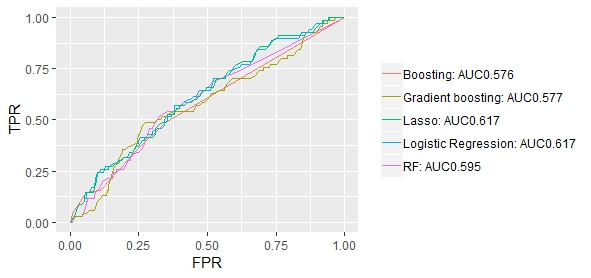
\includegraphics[width=6in]{OriginalFeatures.jpeg}
  \caption{Model performance}
  \label{fig:example} 
\end{figure} 

\subsection{Re-evaluating Performance with New Features} 
We were able to see marginal improvements in performance by adding the two new features. Figures 2 and 3 show the ROC curves and AUC values for the baseline and additional features, respectively. The logistic regression model had the highest AUC value (0.617) using the four baseline features. However, after adding income and number of young children, the gradient boosted forest performed best and had the highest AUC value (0.659). These results are summarized in Table 5.  


\begin{figure}[h]
  \centering 
  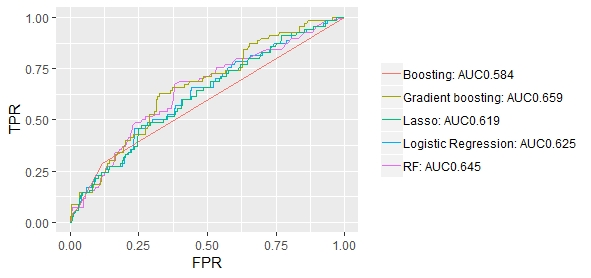
\includegraphics[width=6in]{NewFeatures.jpeg}
  \caption{Model performance with new features}
  \label{} 
\end{figure} 


\section{Results} \label{results}
The original model, logistic regression, used baseline features of gender, age, race, and birth country to predict children's obesity status. Model performance improved when we added two features of annual household income and the number of children 5 years old or younger. The AUC increased from 0.617 to 0.659 as shown in Table 5. However, the best model changed from the logistic regression to the gradient boosted forest. This is not too surprising. Logistic regression is likely to perform comparatively well when the data underlying it are simple. As we increased complexity by adding additional features, the gradient boosted forest (an ensemble method) outperformed the logistic regression. 

However, this improvement is not considerable enough to build the prediction model. One of the possible reasons why the AUC is still less than 0.7 is our sample size. Referring to the previous research, they built large datasets by combining several years worth of survey data to increase the total sample size to 10,000 or more. Also, some of them did not focus on children, which enabled them to have more samples. Appendix A mentions the potential sample size issues further. 

\begin{table}[h]
  \centering 
  \begin{tabular}{lclc} 
    Method & AUC \\ 
    \hline \\[-11pt]
    Gradient Boosting with new features & 0.659 \\
    Logistic Regression (Base model) & 0.617 \\ 
   \hline 
  \end{tabular}
  \label{tab:example} 
    \caption{Outcome by method used. These are our results.} 
\end{table}


\section{Discussion and Related Work} \label{discussion}
Our results demonstrate the ability to boost model performance when the right features are added. However, even with these additional features, the best performing model (the gradient boosted forest) still only had an AUC value of 0.659. This illustrates the limitations of using only demographic data to classify health categories. We expect that many other features play a role in BMI category, including genetics, home environment, diet, etc. But even with demographic information only, this model could still help guide health protection agencies, like the CDC. Understanding the demographic nature of various communities across the country, this model could suggest regions for additional health assistance (e.g. food stamps). Please see Appendix A for a further discussion explaining why our performance might be low.

Many machine learning analyses, including this one, use self-reported survey data to build predictive models. However, rich new sources of health data are coming online. \cite{degreg:18} discuss these sources, which include sensors, smartphone apps, electronic medical records and insurance recordings. These sources not only provide more abundant and accessible health data, but also more accurate data. With these new data comes the opportunity for more advanced machine learning analyses, using such algorithms as random forests and deep neural networks. 

Future research should consider using fresh sources of health data, such as data collected from Fitbits, to perform innovative machine learning analyses. Given that  private companies tend to collect the most accurate, large-scale data, government health agencies should consider public-private partnerships with these companies to obtain the highest quality, most recent data.

Furthermore, agencies like the CDC should consider expanding their surveys to include more participants. The model built in our study, while informative, did not have particularly high performance, as measured by AUC. Part of this low performance could be attributed to the small sample size of the training data. Given it is costly to obtain additional survey results, we suggest the CDC consider other, cheaper methods of collecting health data online, through phone applications, or by establishing public-private partnerships. Additionally, future work should consider including additional, helpful features in the model-building process. 


\section{Conclusion} \label{conclusion}
We used the study performed by \cite{kaur:17} as our launch point for this application. Our study applies sophisticated machine learning methods - logistic regression, regularized logistic regression (lasso), random forest, boosted forest and gradient boosted forest - to demographic data from the CDC's NHANES National Youth Fitness Survey from 2012. The goal was to classify obese children (with the outcome created from BMI category data, which was recorded from examinations) using only basic demographic features: gender, age, race and birth country. We demonstrated improvements in model performance by adding two demographic features to the baseline model: income and number of young children in the household. Even though our best model's performance only peaked at an AUC value of 0.659, this application study demonstrates the ability of the machine learning pipeline to provide value and insights to government health agencies. This study should serve as a foundational step towards bringing innovative machine learning techniques to the forefront in public sector survey analyses.


%ACKNOWLEDGEMENTS
%\acks{Many thanks to all collaborators and funders!}

\bibliography{ML_Project_References.bib}  % Should contain at least 10 cited references

\appendix
\section*{Appendix A.}\label{aa}
\cite{kaur:17} used data from 9,701 survey participants from 2001 to 2010. To obtain enough data, they combined survey results from five survey cycles. Our study, on the other hand, uses data from a special one-time survey, called the NHANES National Youth Fitness Survey (NNYFS). Given the special nature of this survey, we were only able to build our models using data from 1,526 participants without missing data. We believe this small amount of data contributed to our relatively low AUC values. 

\section*{Appendix B.}\label{ab}
While only 5 participants were missing the outcome of interest, BMI category, other participants were missing values for covariates. Since we only had a few missing values for annual household income (45), we did not impute these missing values for the final model. At first, we performed multiple imputation on the missing variables using R's mice package. However, when comparing model performance {\em with} the imputed values to model performance {\em without} the imputed values, the difference was negligible or nonexistent. The AUC values for a few of the models improved marginally, by only 0.001. While multiple imputation is a helpful and reliable method to address missing data, imputation in survey data is still ill-advised.

\cite{wl:19} discuss additional novel ways to handle missing data. However, they, too, suggest avoiding imputation when the number missing is small. \cite{curley:19} perform comparative analyses on various techniques to handle missing data in surveys. They demonstrate that multiple imputation, when used on a supported set of predictor variables, can yield benefits. But these benefits are really only noticeable when there is a {\em large degree of missingness.} We did not consider less than 50 rows of missing data to count as a large degree. Understanding the challenges of imputation, we selected predictor variables with relatively few missing values to use in our models.

\section*{Appendix C.}\label{ac}
In addition to the models mentioned above, we also implemented a neural network model. Unfortunately, it did not give us a better prediction model probably likely due to the limited number of samples. But we were able to show how to implement a neural network model with our data set.

First, we created dummy variables that fit the neural model input format. Then, we created the model composed of the input layer, two hidden layers and the output layer. We decided that regularization was not necessary for our case based on the exploration of models and features above, since most of the coefficients are not regularized with lasso. Therefore, we used ReLU activation, which is the most common activation function, for the input layer and two hidden layers without regularization. Since our purpose is classification, for the output layer, we used the sigmoid function. We used mean squared error to optimize the model. After that, we trained the model until it reached the stopping criteria, defined as the local minimum. When we saw the predictions, all of them were classified as 1, which indicated the prediction did not work well. Similar to the  discussion above, it is suggested our sample size is too small and the predictors too simple to use a neural network for this task.

\end{document}